% ЕМТ 2022, VI клас — точен LaTeX препис от официалните файлове в Klasirane.com.
% Условия: https://klasirane.com/api/competitions/EMT/All/2022/6%20%D0%BA%D0%BB/probs
% SHA-256 (условия): ec53e632b8af1d0e61024e0e4c9375e998b7842dacd7d79155c83914de565728
% Решения: https://klasirane.com/api/competitions/EMT/All/2022/6%20%D0%BA%D0%BB/sol
% SHA-256 (решения): d8f568b8ec83e374e95522131866df098123ce4e5fbc5bcd0dc0903887194c4d
% Точковите оценки, правописът, формулировките и видимите печатни особености са запазени от източника.
% Фигурите са неизменни изрези от официалните PDF файлове, изобразени с 3 пиксела на PDF точка.

Задача 6.1. Две мравки се движат по числовата ос. В началото те се намират в точките, които съответстват на числата $a$ и $b$, $b>a$. На втория ден се преместват съответно в точките $2a-b$ и $2b-a$ и продължават по същия начин: от точките $x$ и $y$ на следващия ден преминават съответно в точките $2x-y$ и $2y-x$.

а) Ако
$$
a=-39\frac{3}{13}\cdot23\frac{11}{28}+3\frac{3}{13}:\frac{4}{11}+39\frac{3}{13}\cdot20\frac{9}{14},
$$
$$
b=\frac{1}{20+\dfrac{1}{1+\frac{1}{10}}}:\left(\frac{1}{9\cdot11}-\frac{1}{10\cdot12}+\frac{1}{11\cdot13}-\frac{1}{12\cdot14}+\cdots+\frac{1}{43\cdot45}-\frac{1}{44\cdot46}\right),
$$
коя точка от числовата ос ще се намира на равни разстояния от двете мравки на петия ден?

б) Намерете числата $a$ и $b$, които определят първоначалните позиции на мравките, ако на петия ден разстоянието между мравките е било 2025, а на десетия ден те са били на равни разстояния от точката $-2022$.

Решение. Дължината на отсечка с краища в числата $a$ и $b$ е $b-a$. Средата на отсечката е в точката $a+\dfrac12(b-a)=\dfrac12(a+b)$. Забелязваме, че $(2a-b)+(2b-a)=a+b$, което означава, че сборът на числата от двете граници се запазва. Следователно средата на отсечката с краища в двете мравки не се променя.

а) Намираме
$$
a=-39\frac{3}{13}\cdot\left(23\frac{11}{28}-20\frac{9}{14}\right)+3\frac{3}{13}\cdot\frac{11}{4}=
$$
$$
=-39\frac{3}{13}\cdot2\frac{3}{4}+3\frac{3}{13}\cdot\frac{11}{4}=\left(-39\frac{3}{13}+3\frac{3}{13}\right)\cdot\frac{11}{4}=-36\cdot\frac{11}{4}=-99.
$$

Делимото в $b$ е равно на $1:\left(20+1:\dfrac{11}{10}\right)=1:20\dfrac{10}{11}=\dfrac{11}{230}$.

Като използваме равенството
$$
\frac{2}{n(n+2)}=\frac1n-\frac{1}{n+2},
$$
намираме
$$
\frac{1}{9\cdot11}+\frac{1}{11\cdot13}+\cdots+\frac{1}{43\cdot45}=\frac12\left(\frac19-\frac{1}{45}\right)=\frac{2}{45}
$$
и
$$
\frac{1}{10\cdot12}+\frac{1}{12\cdot14}+\cdots+\frac{1}{44\cdot46}=\frac12\left(\frac{1}{10}-\frac{1}{46}\right)=\frac{9}{230}.
$$

Тогава
$$
b=\frac{11}{230}:\left(\frac{2}{45}-\frac{9}{230}\right)=\frac{11}{230}:\frac{11}{230\cdot9}=9.
$$

Средата на отсечката е в точката $\dfrac12(a+b)=\dfrac12\cdot(-99+9)=-45$.

б) Имаме $\dfrac12(a+b)=-2022$, т.е. $a+b=-4044$.

Тъй като $(2b-a)-(2a-b)=3(b-a)$, всеки следващ ден дължината на отсечката се утроява. Следователно на петия ден тя е $3^4\cdot(b-a)=2025$ и $b-a=25$.

Намираме $2b=(a+b)+(b-a)=-4019$ и $b=-2009,5$, както и $2a=(a+b)-(b-a)=-4069$ и $a=-2034,5$.

Критерии за оценяване.

а) 3 точки (за намиране на $a$ и на $b$ по 1 точка; за намиране на средата – 1 точка); б) 3 точки; (за доказване, че дължината на интервала се утроява всеки ден – 1 т.; за доказване, че средата се запазва – 1 т.; за намиране на $a$ и $b$ – 1 точка)

Задача 6.2. В съкровището на дракона Мог има четири вида скъпоценни камъни: 50\% от скъпоценните камъни и още един са изумруди, 60\% от останалите камъни и още четири са рубини, 55\% от камъните без изумрудите и рубините са аметисти, а останалите 180 камъни са диаманти.

А) Колко скъпоценни камъни има в съкровището на Мог?

Б) Джуджетата Крор, Фрор и Дрор, заедно с Билбо, откраднали съкровището на дракона и си го поделили. Скъпоценните камъни на Крор били с 24\% повече от тези на Фрор, а Дрор взел с 25\% по-малко камъни, отколкото Крор и Фрор общо. Най-малко колко скъпоценни камъни е взел Билбо?

Решение. а) Разсъждаваме отзад напред: 180 диаманта са 45\% от общия брой на диамантите и аметистите, следователно диамантите и аметистите са общо $180:0,45=400$; $400+4=404$ камъни са 40\% от общия брой рубини, аметисти и диаманти, следователно рубините, аметистите и диамантите общо са $404:0,4=1010$. Половината от всички камъни са $1010+1=1011$, следователно в съкровището има 2022 камъни.

б) Броят камъни на Крор е $124\%=\dfrac{31}{25}$ от броя камъни на Фрор. Тъй като броят на камъните е естествено число, то броят на камъните на Фрор се дели на 25, т.е. е от вида $25x$, където $x$ е естествено число. Тогава Крор има $31x$ камъни, а Дрор има $75\%\cdot(25x+31x)=42x$ камъни. Общо трите джуджета имат $25x+31x+42x=98x$ камъни. Тъй като $2022:98=20$ (ост. 62), то Билбо е взел най-малко 62 скъпоценни камъни.

Критерии за оценяване.

а) 3 точки; за оценка – 3 т., б) 3 точки; включително ако задачата е решена вярно при друг общ брой на камъните.

Задача 6.3. Даден е изпъкнал четириъгълник $ABCD$. Страните му $AB$, $BC$, $CD$ и $DA$ са продължени съответно до точките $M$, $N$, $P$ и $Q$ така, че $AB=BM$, $BC=CN$, $CD=DP$ и $DA=AQ$. Лицето на четириъгълника $MNPQ$ е 250 cm$^2$.

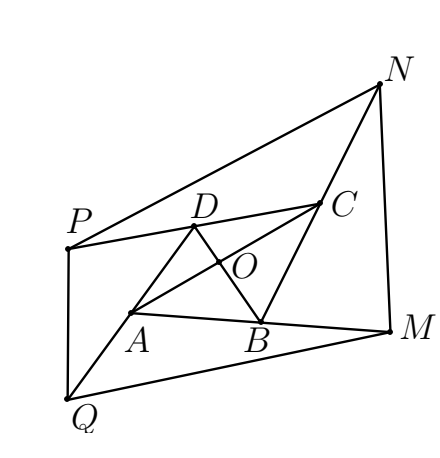
\includegraphics[max width=0.42\textwidth, alt={Четириъгълниците ABCD и MNPQ с пресечна точка O на диагоналите}, center]{assets/6-3-figure.png}

а) Да се намери лицето на $ABCD$.

б) б) Диагоналите на четириъгълника $ABCD$ се пресичат в точка $O$. Намерете лицата на триъгълниците $AOB$, $BOC$, $COD$ и $DOA$, ако е известно, че стойностите им (в квадратни сантиметри) са прости числа.

Решение. В триъгълник $AMC$ отсечката $CB$ е медиана. Следователно $S_{ABC}=S_{MBC}=\dfrac12S_{AMC}$.

В триъгълник $BMC$ отсечката $MC$ е медиана. Следователно $S_{BMC}=S_{NMC}=\dfrac12S_{BMN}$.

Следователно $S_{ABC}=S_{MBC}=S_{NMC}$ и
$$
2S_{ABC}=S_{MBC}+S_{NMC}=S_{BMN}.
$$

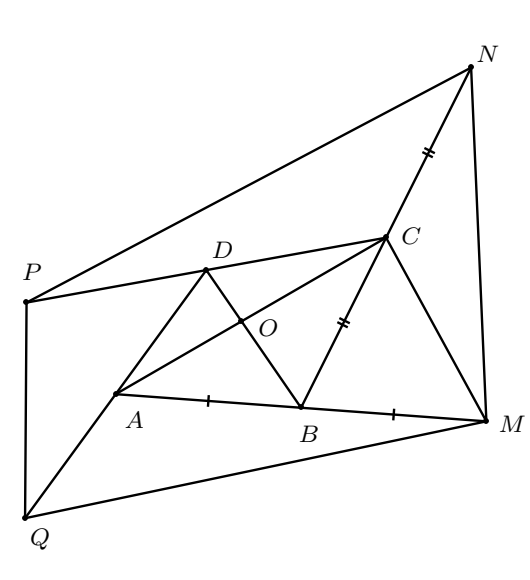
\includegraphics[max width=0.48\textwidth, alt={Четириъгълниците ABCD и MNPQ с означени равни отсечки}, center]{assets/6-3-solution-figure.png}

Аналогично $2S_{BCD}=S_{CNP}$, $2S_{CDA}=S_{DPQ}$, $2S_{DAB}=S_{AQM}$. Събираме равенствата и получаваме
$$
2(S_{ABC}+S_{BCD}+S_{CDA}+S_{DAB})=S_{BMN}+S_{CNP}+S_{DPQ}+S_{AQM},
$$
$$
4S_{ABCD}=S_{BMN}+S_{CNP}+S_{DPQ}+S_{AQM}.
$$

От тук следва, че $5S_{ABCD}=S_{MNPQ}$. Следователно $S_{ABCD}=50$ cm$^2$.

б) Да означим $S_{AOB}=S_1$, $S_{BOC}=S_2$, $S_{COD}=S_3$, $S_{DOA}=S_4$. Тогава $S_1+S_2+S_3+S_4=S_{ABCD}=50$.

Триъгълниците $AOB$ и $AOC$ имат обща височина $h_b$ през върха $B$. За лицата им е вярно
$$
\frac{S_1}{S_2}=\frac{\frac12AO\cdot h_b}{\frac12OC\cdot h_b}=\frac{AO}{OC}.
$$
Аналогично $\dfrac{S_4}{S_3}=\dfrac{AO}{OC}$. Следователно $\dfrac{S_1}{S_2}=\dfrac{S_4}{S_3}$ или $S_1\cdot S_3=S_2\cdot S_4$.

Тъй като $S_1$, $S_2$, $S_3$ и $S_4$ са прости числа, а съществува единствено разлагане на прости множители на числото $S_1\cdot S_3$, то $S_1=S_2=p$ и $S_3=S_4=q$ или $S_1=S_4=p$ и $S_3=S_2=q$, където $p$ и $q$ са прости числа. Заместваме в равенството $S_1+S_2+S_3+S_4=50$ и получаваме, че $p+q=25$. Това означава, че $p$ и $q$ са от различна четност и тъй като $p$ и $q$ са прости числа, то едното от тях е задължително 2, а за другото остава 23. Като обобщим резултатите се получават 4 възможни решения:
$$
S_{AOB}=2,\ S_{BOC}=2,\ S_{COD}=23,\ S_{DOA}=23;
$$
$$
S_{AOB}=2,\ S_{BOC}=23,\ S_{COD}=23,\ S_{DOA}=2;
$$
$$
S_{AOB}=23,\ S_{BOC}=2,\ S_{COD}=2,\ S_{DOA}=23;
$$
$$
S_{AOB}=23,\ S_{BOC}=23,\ S_{COD}=2,\ S_{DOA}=2.
$$

Критерии за оценяване.

а) 4 точки; б) 3 точки.

Задача 6.4. Правоъгълник с дължина, която е два пъти по-голяма от широчината, наричаме домино. На чертежа е показано как всеки квадрат може да се разреже на пет домина.

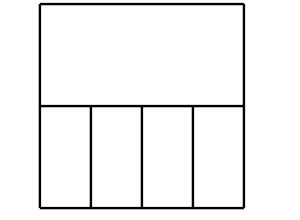
\includegraphics[max width=0.28\textwidth, alt={Квадрат, разрязан на пет домина}, center]{assets/6-4-five-dominoes.png}

а) Посочете пример как квадрат може да се разреже на шест домина и как може да се разреже на седем домина.

б) Посочете пример как квадрат може да се разреже на шест домина, сред които има поне четири с различни размери.

в) Докажете, че за всяко естествено число $n$, по-голямо от 7, квадратът може да се разреже на $n$ домина.

Решение. а) На чертежа са показани два примера за разрязване на шест домина

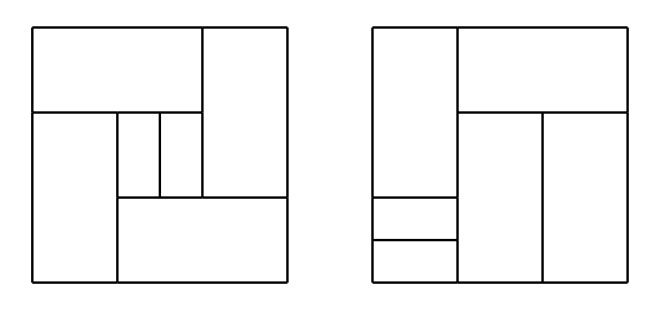
\includegraphics[max width=0.56\textwidth, alt={Два примера за разрязване на квадрат на шест домина}, center]{assets/6-4-six-examples.png}

и два примера за разрязване на седем домина.

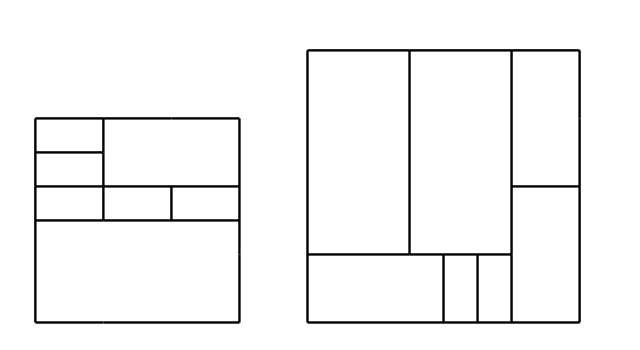
\includegraphics[max width=0.56\textwidth, alt={Два примера за разрязване на квадрат на седем домина}, center]{assets/6-4-seven-examples.png}

б) На чертежа е показано как квадрат $8\times8$ може да се разреже на едно домино $4\times8$, едно домино $3\times6$, едно домино $2\times4$ и три домина $1\times2$.

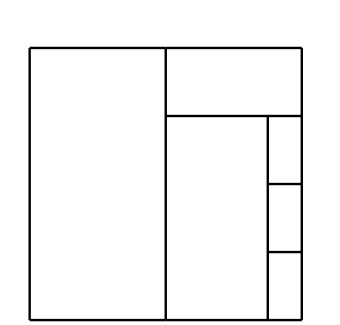
\includegraphics[max width=0.30\textwidth, alt={Квадрат осем по осем, разрязан на шест домина с четири различни размера}, center]{assets/6-4-four-sizes-example.png}

б) В условието е показано как квадрат може да се разреже на 5 домина, а в а) е показано как квадрат може да се разреже на 6 или 7 домина.

Остава да забележим, че всяко домино може да се разреже на 4 домина. С такова разрязване броят на домината се увеличава с 3.

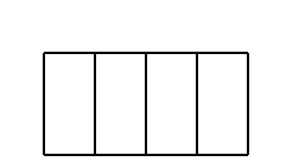
\includegraphics[max width=0.28\textwidth, alt={Домино, разрязано на четири по-малки домина}, center]{assets/6-4-subdivision.png}

Следователно от примера с 5 домина след $k$ разрязвания се получава разрязване на $5+3k$ домина; от примера с 6 домина след $k$ разрязвания се получава разрязване на $6+3k$ домина; от примера със 7 домина след $k$ разрязвания се получава разрязване на $7+3k$ домина. Всяко естествено $n\geq8$ попада в един от тези случаи.

Критерии за оценяване.

а) 2 точки; (по две за пример); б) 2 точки; в) 3 точки.
